\section{Mission operations \& timeline}\label{cha:opseg}
This chapter describes the mission operational segment, giving an overview of mission phases and related activities. It serves to identify the actions to be performed by the system over the mission duration. It is essential that these are taken into account in mission design for a complete and feasible mission. To this end, the mission is divided into four phases: 
\begin{itemize}
\item[I]{Interplanetary flight up to the sphere of influence}
\item[II]{Re-entry from the sphere of influence to the point of atmospheric entry}
\item[III]{Re-entry from the point of atmospheric entry to the terminal point at 10 kilometres altitude}
\item[IV]{Final descent from the terminal point at 10 kilometres altitude to ground level}
\end{itemize}
These four phases are discussed hereafter in sections \ref{sec:p1}-\ref{sec:p4} and are also graphically displayed in Fig. 

\begin{figure}[H]
\centering
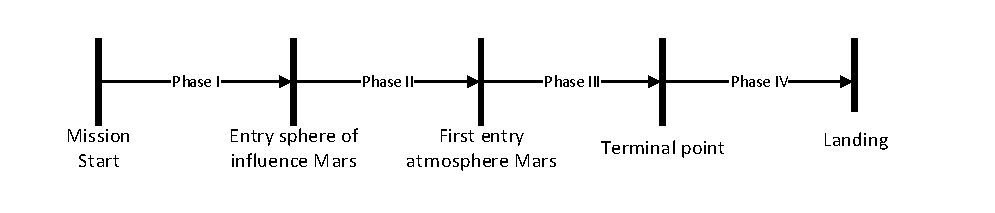
\includegraphics[width = 1.0\textwidth]{Figure/OPS.pdf}
\caption{Timeline of mission phases}
\label{fig:time}
\end{figure}

\subsection{Phase I}\label{sec:p1}
The first phase imposes the following requirements on the vehicle:
\begin{itemize}
\item The payload shall provide sufficient volume and adequate living capability for human payload. Since the mission strictly only concerns the re-entry part, the relevance of this mission phase is mainly to impose human payload requirements. 
\item  The mission requires use of a launcher. The launcher limits the maximum diameter of the re-entry vehicle as well as its mass, since it is more economically feasible to adhere to current launcher availabilities rather than to develop a new launcher.
\end{itemize}
Moreover, transfer time should be within the limits of human payload endurance. As such, a Hohmann transfer is not a feasible option due to its large transfer time and a higher energy transfer orbit is more realistic. This affects how Mars is approached.

\subsection{Phase II}\label{sec:p2}
The start of the second mission phase signifies the initiation of control system activities in trajectory control. Phase II starts when the sphere of influence of Mars is reached.  At this point the descent towards the surface of Mars is nearing after a long transfer. Communication  with the groundstation is intensified at this point. Communication delays have become quite significant and in the order of minutes depending on the relative positions of Mars with respect to the earth.  
During this stage the spacecraft is accelerated towards Mars and further controlled to reach the atmosphere at the design entry point of this mission. 

\subsection{Phase III}\label{sec:p3}

Phase three starts with the deployment of the decelerator system. The aeroshell deployment is dependent on the design concept chosen and is summarized below for each of the concepts 

\begin{itemize}
\item Tension cone, stacked toroid, trailing: These inflatable concepts are best inflated just before the first entry of the spacecraft into the Martian atmosphere. The deployment is performed by releasing a pressurized gas into the inflatables
\item Isotensoid: The isotensoid design is inflated by ram air. At the first entry of the atmosphere the deployment system may be released but the decelerator is not yet deployed. This is a time dependent function following the inflow of ram-air into the system. For this deployment it is required that the spacecraft is already into the atmosphere.
\item Rigid: The rigid concept features no deployment mechanism
\end{itemize}

This phase consist of extensive communications to earth, considering however that control from earth is not possible during the atmospheric entry due to the long round trip time. After the first exit from the Martian atmosphere progress may be communicated between the ground station and the spacecraft for the next re-entry still considering the long round trip times. In principle however the re-entry vehicle should be self sufficing.

The primary operations in this phase of the missions are those of the control system. .... nu verder

\subsection{Phase IV}\label{sec:p4}
The final descent phase employs deployment mechanisms other than the inflatable aeroshell and demands a high precision in landing at a designated landing site. To this end, the terminal conditions with which the third phase is exited affect the final descent. To avoid requirements on aerodynamic braking in the final descent phase from being overly demanding, from this phase the requirement flows down that at the terminal altitude of 10 [km] the terminal Mach number shall not exceed 5 [-]. 

